\subsection{Two-dimensional ring dataset }

\begin{figure}
  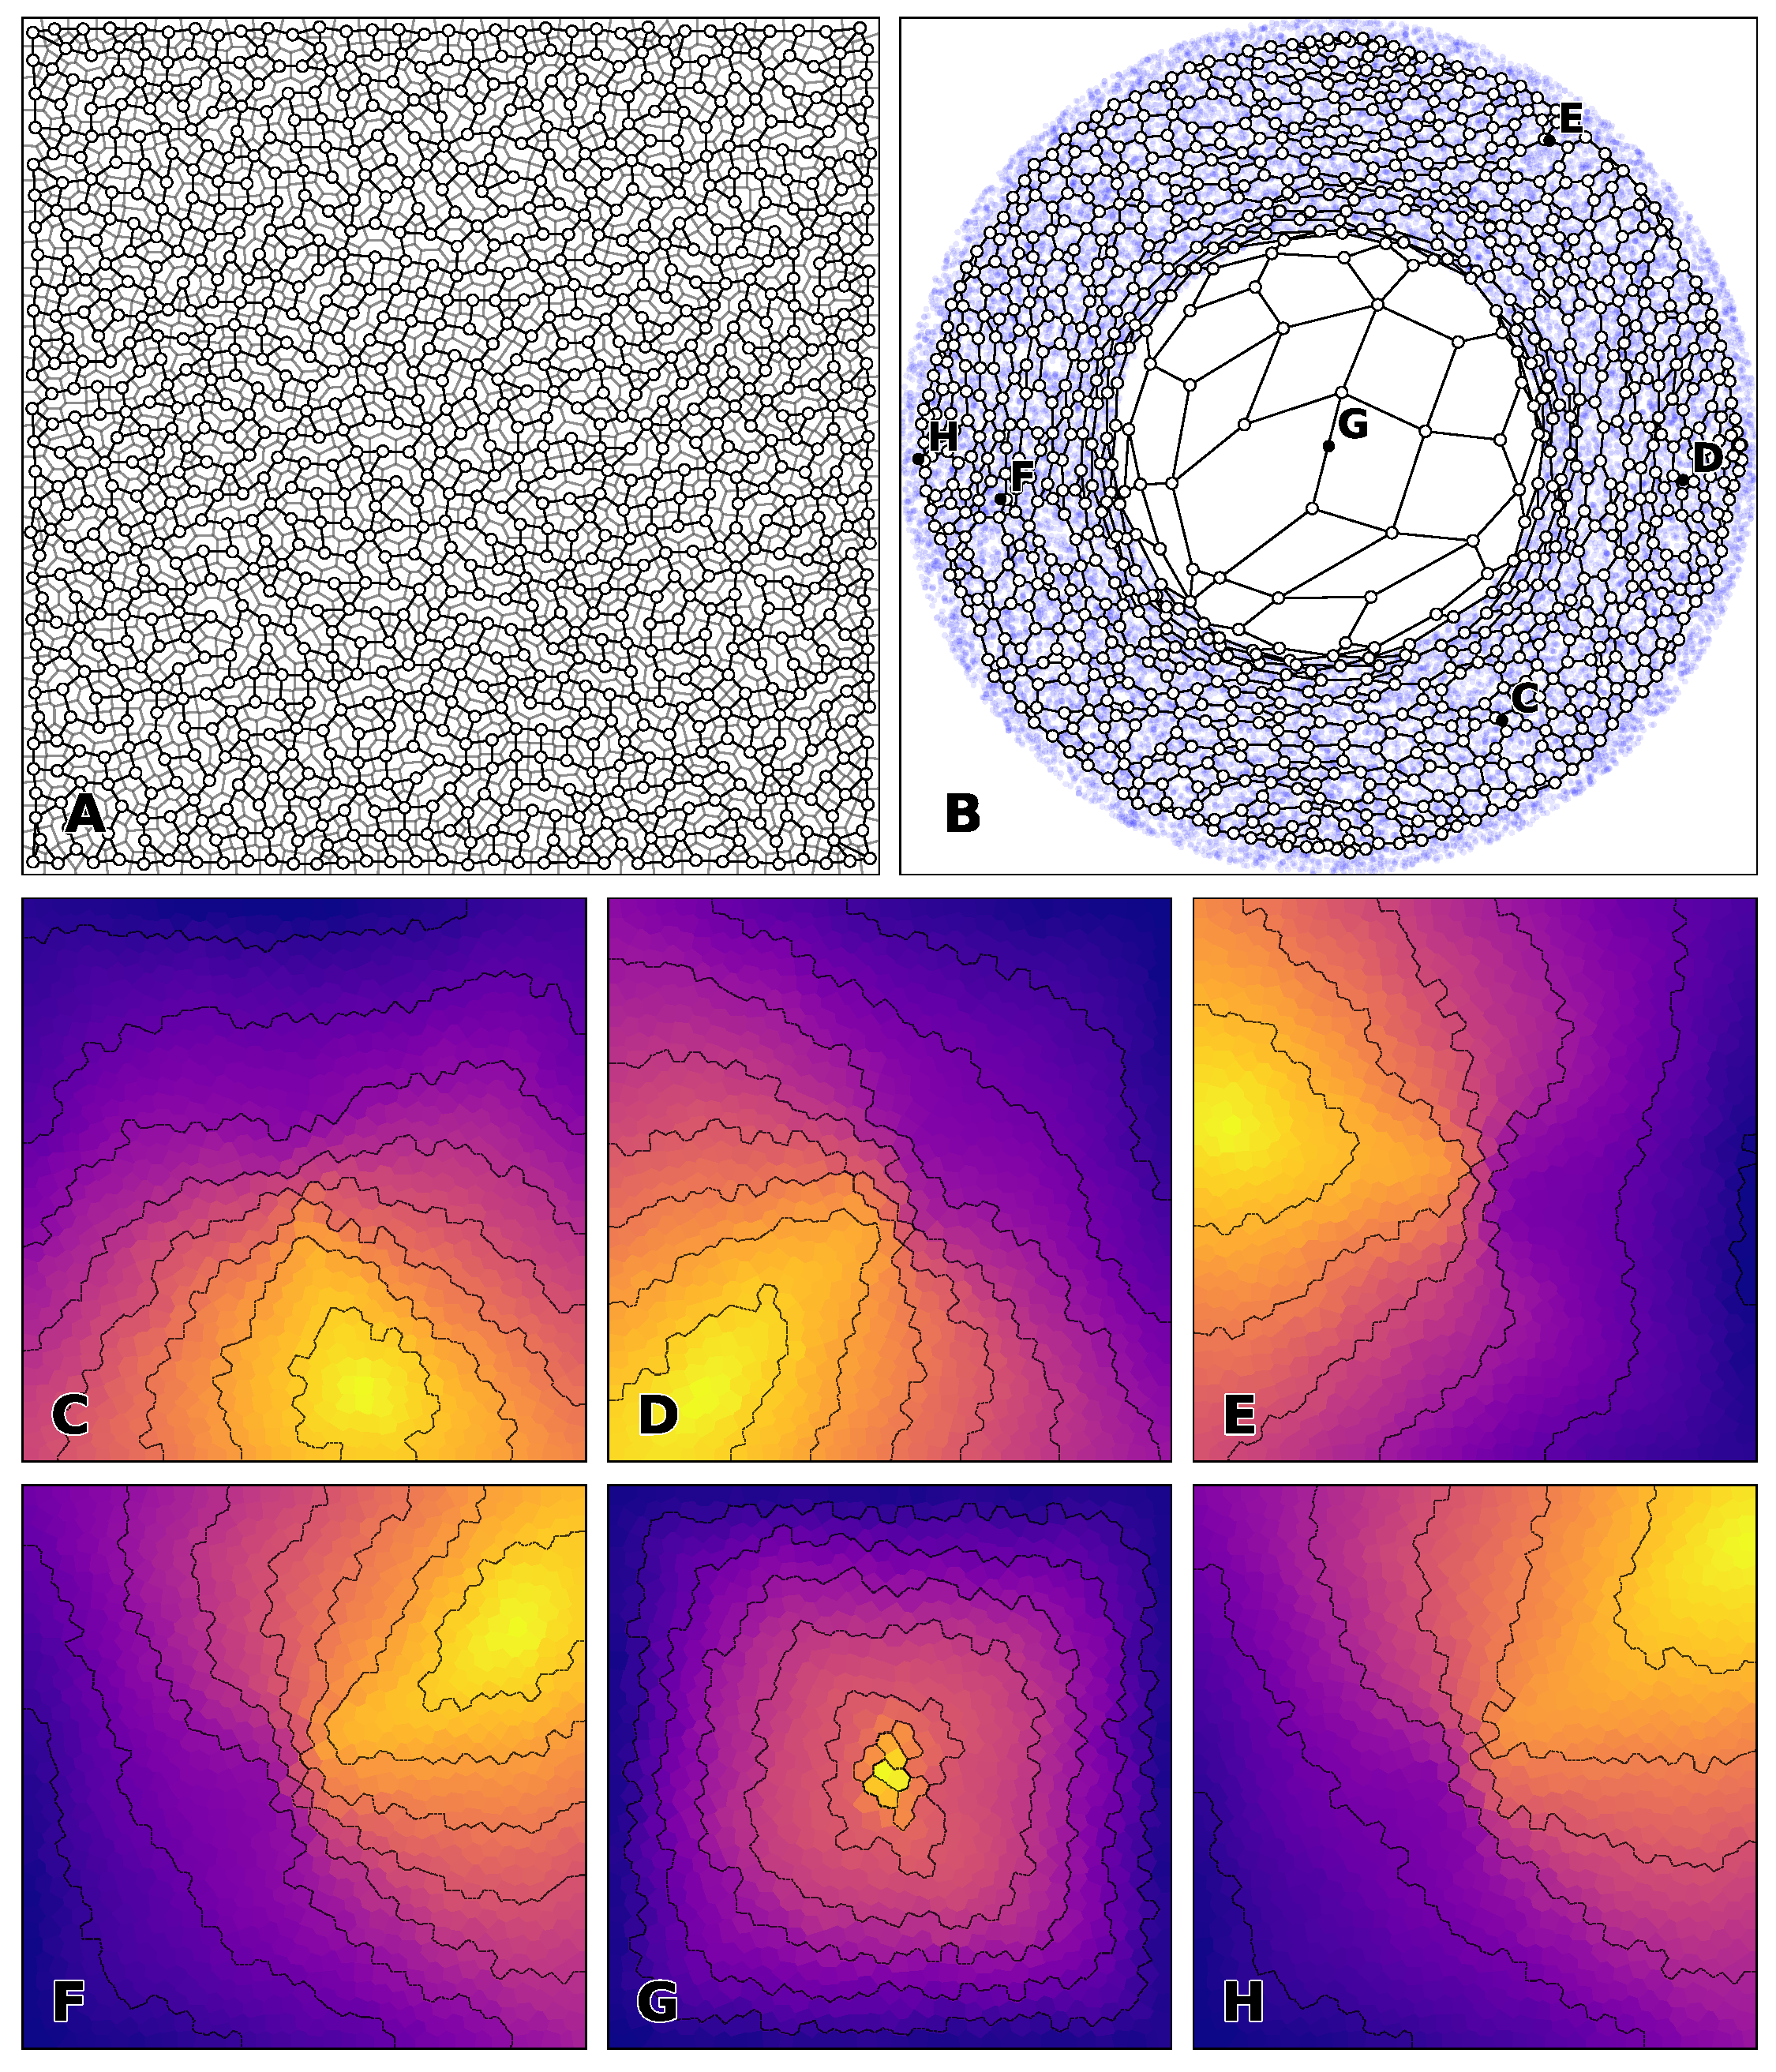
\includegraphics[width=\columnwidth]{experiment-2D-torus.pdf}
  \vspace{2mm}
  \centering
  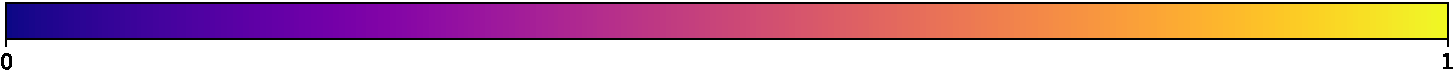
\includegraphics[width=.975\columnwidth]{figures/colormap.pdf}
  %
  \caption{%
  %
  {\bfseries \sffamily Two dimensional ring dataset (results)}
  %
  Randomized SOM made of $1024$ neurons with a $3$-nearest neighbors induced topology. Model has been trained for $25,000$ epochs on two-dimensional points drawn from a ring distribution on the unit square. \textbf{A} Map topology in neural space. \textbf{B} Map topology in data space. \textbf{C to H} Normalized distance map for six samples. Normalization has been performed for each sample in order to enhance contrast but this prevents comparison between maps.
  %
  }
  \label{fig:2D-ring:results}
\end{figure}


% A one-dimensional problem as the one in the previous paragraph does not reveal a lot of information with respec to the organization of the map. Therefore, we proceed with investigating how a two-dimensional map learns two-dimensional representations. First, we train the SOM algorithms (both the Kohonen and VSOM) on $25000$ two-dimensional points drawn from a uniform distribution of an annulus in $[0, 1]\times[0, 1$]. More precisely, $x_1 = \frac{1 + r \cos(k)}{2}$ and $x_2 = \frac{1 + r\sin(k)}{2}$, where $k \sim \mathcal{U}(0, 2\pi)$ and $r \sim \sqrt{\mathcal{U}(\frac{1}{4}, 1)}$. After placing the neurons on the appropriate positions on neural space with respect to the topology provided by a blue noise distribution (only for the VSOM algorithm), we train the maps for $25000$ epochs. Both Kohonen and VSOM algorithms use $1024$ neurons. The results after convergence are shown in Figure~\ref{fig:annulus}, where the map topology of the annulus is shown in Figure~\ref{fig:annulus}{\bfseries \sffamily A}. The mapping produced by the VSOM learning algorithm is shown in Figure~\ref{fig:annulus}{\bfseries \sffamily B} trained on the annulus data set. As we observe the map covers the input space with higher density within the annulus, where the input data points lie, and a lower density within the hole of annulus. Panels~\ref{fig:annulus}{\bfseries \sffamily C}-{\bfseries \sffamily H} display the responses of six neurons (see the red annotated points in panel~\ref{fig:annulus}{\bfseries \sffamily B}) to a stimulus derived from  the discretization of $[0, 1]\times [0, 1]$. The responses of these neurons are well organized and reflect their receptive fields. 

% The distribution of eigenvalues for the two maps (black and blue colors correspond to VSOM and Kohonen maps, respectively) for the current experiment are shown in Figure~\ref{Fig:distributions}{\bfseries \sffamily A}. We observe that there is no significant difference between the two distributions and thus the two algorithms perform equally (see Section~\ref{sec:gram} for more details about how we obtain the distributions). Also the Wasserstein distance indicates that the two distributions are almost identical. 

% Finally, the persistence barcodes and diagrams in Figure~\ref{Fig:persistence_exp2} indicate that the Kohonen map (middle column in the figure) does not capture so well the $H1$ topological features of the input (first column in the figure),  although it captures the $H1$ properties. This is related to the fact that the  Kohonen map covers with more neurons the hole of the annulus which is not  the case with the VSOM. VSOM retains better than Kohonen the $H1$ topological features and this is reflected in the barcode and diagram (last column) where the blue dots resemble the cluster of blue dots of input's diagram (first column). This indicates that VSOM uses less neurons to cover the hole of the annulus, which can be confirmed by visually inspecting Figure~\ref{fig:annulus}{\bfseries \sffamily B}. The same phenomenon is present in the persistent barcodes where the blue segments appear in input's and VSOM's barcodes but not as strongly as in Kohonen's. 
